\chapter{Eine Anwendung für mobiles Maschinelles Lernen}
\label{chap:application}
Es konnten bis hierher bereits einige Kenntnisse gewonnen
werden. Wir haben die Grundlagen von Deep Learning untersucht
und den Prozess beschrieben, wie mit TensorFlow und Keras
ein neuronales Netz erstellt und trainiert werden kann.
Das Modell wurde in ein mobil- und TPU-kompatibles Format umgewandelt
und anschließend miteinander vergleichen.
Hierbei konnte das Ergebnis festgehalten werden,
dass zumindest bei kleinen Modellen und bestimmten Netzarchitekturen
die Inferenzgeschwindigkeit
auf der Edge TPU nicht unbedingt schneller ist als die gleiche Ausführung auf der CPU.
Ein neuronales Netz allein, welches hervorragende Prognosen
macht, reicht jedoch nicht, um ein nützliches Produkt zu entwickeln:
Das Modell muss in einer Anwendung integriert werden, sodass
der Benutzer oder andere Teile des Systems
mit den Modellergebnissen interagieren können.
Der Entwurf einer solchen Anwendung ist die
Fokussierung dieses Kapitels.

\section{Die allgemeine Architektur auslegen}
Wie in \autoref{sec:problem-description} beschrieben wurde, ist es
typischerweise eine gute Idee, das Modell in einen Service zu verpacken.
Andere Teile der Anwendung können so jederzeit auf die Vorhersagen
des Netzes zugreifen. Dies ermöglicht es, neue Versionen
einzuspielen, ohne die Hauptanwendung zu unterbrechen.
Zusätzlich kann die Entwicklung flexibler gestaltet werden,
da es keine Einschränkung auf bestimmte Technologien
und Programmiersprachen gibt. Es kann so jederzeit das
beste Werkzeug für das zu lösende Problem ausgewählt werden.
Der Service, der das Modell ausführt, könnte in Python oder \cpp{}
geschrieben sein, und obwohl es möglich ist, Benutzeroberflächen 
in Python zu entwerfen, ist \cpp{} wahrscheinlich nicht das
richtige Hilfsmittel für diese Aufgabe.
Besser wäre es womöglich eine Sprache für das Web auszuwählen, 
wie zum Beispiel JavaScript.
\autoref{fig:app-architecture} zeigt die Architektur der Anwendung.
\begin{figure}[h!]
  \centering
  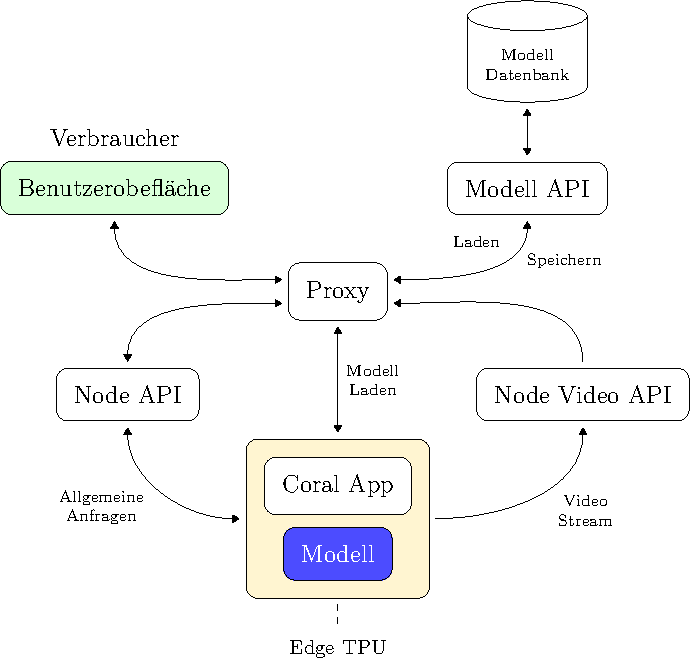
\includegraphics[width=\wLG]{app/app-architecture.pdf}
  \caption{Die Architektur der Anwendung: Ein Modell, das als Dienst
  bereitgestellt wird und verschiedene Services, die mit diesem kommunizieren}
  \label{fig:app-architecture}
\end{figure}

\noindent
Jedes Objekt mit einer Pfeilspitze spiegelt einen Service wieder, insgesamt sind
es sieben Stück. Ein Service ist eine unabhängige, wenn möglich kleine und
unkomplizierte Anwendung, welche nicht mehr als eine Aufgabe übernimmt.
Um die Verwaltung dieser Services zu erleichtern, wird Docker eingesetzt.
Jeder Dienst kann so isoliert in seinem eigenen Docker-Container ausgeführt
und über Docker-Netzwerke verbunden werden.\\[8pt]
Docker ist eine Freie Software, welche auf Linux, Windows und macOS
läuft. Sie erstellt und verwaltet Container
und kann diese sogar orchestrieren.
Docker, Inc., gegründet in 2008 (ursprünglich \textit{dotCloud} und später unter
dem Spitznamen \enquote{Docker}), ist das Unternehmen,
welche die Software entwickelt hat \parencite{onlide:docker-inc}.
Das Wort \enquote{Docker} kommt aus dem Englischen
und bedeutet \textit{\underline{dock} work\underline{er}} --
eine Person im Hafen die Schiffe be- und entlädt.
Es ermöglicht das einfache Teilen von Software
durch Docker-Images (einschließlich aller Abhängigkeiten
und in der Regel geeigneter Standardkonfiguration) und kann
diese mithilfe der Docker-Engine ausführen.
Wird ein Image ausgeführt, erstellt die Engine einen Docker-Container,
mit dem die Anwendung gut isoliert vom restlichen System gestartet wird.
Es ist ähnlich wie eine virtuelle Maschine,
nur viel schneller und schlanker, 
da der Container direkt auf dem Kernel des Hostbetriebssystems aufsetzt
\parencite[11-14]{book:docker-dd} \parencite[672]{book:hands-on-ml}.\\[8pt]
Docker eignet sich somit gut, um eine Anwendung mit der in dieser Arbeit beschriebenen
Zielsetzung zu entwickeln, die jeder herunterladen und mit ein paar Befehlen
auf dem eigenen System ausführen kann. Der Quelltext zur Anwendung
sowie die bisherigen Programme und nicht immer vollständig gezeigten
Ausschnitte, um den Großteil der Abbildungen zu erzeugen,
befinden such auf dem GitHub-Profil des Autors.
Die Docker-Images der in \autoref{fig:app-architecture} zu sehenden
Services sind über Docker Hub verfügbar.
Docker Hub ist eine Plattform zum Teilen von Docker-Images und das als Standard
eingestellte Image-Register einer neuen Installation der Docker Software.
Ein Image-Register enthält ein oder mehrere Image-Repositorys
und diese enthalten wiederum ein oder mehrere Images.
Die folgenden Punkte fassen die wichtigsten Links zusammen:
\begin{itemize}
  \item Der Quelltext zur Anwendung auf GibHub
        (\url{https://github.com/JensDll/coral-ml}).
  \item Die bisherigen Programme und Ausschnitte zum Erstellen der Abbildungen
        (\url{https://github.com/JensDll/bachelorarbeit-notebooks}).
  \item Die Docker-Images der Services auf Docker Hub
        (\href{https://hub.docker.com/repository/docker/jensdll/coral-ml}
        {https://hub.docker.com/reposito\allowbreak ry/docker/jensdll/coral-ml}).
\end{itemize}

\section{Herunterladen der Dienste}
Um ein Image von Docker Hub herunterzuladen, wird
der \consoleinline{docker pull} Befehl verwendet.
Für offizielle Image-Repositorys nimmt dieser Befehl die folgende Form an:
\begin{consolecode}
$ docker pull <repository>:<tag>
\end{consolecode}
Es wird das Repository zusammen mit dem gewünschten Image
in der Form eines Tags angegeben.
Offizielle Repositorys sind ein Prinzip von Docker Hub.
Hier befinden sich von Docker Inc. ausgewählte
Images, die speziell geprüft, getestet,
gut dokumentiert und sicher sein sollten.
Die meisten populären und etablierten Anwendungen
und Betriebssysteme haben ihre eigenen
offiziellen Repositorys auf Docker Hub.
Diese sind Teil der obersten Ebene des Docker Hub Namensraums.
Das Abrufen von Images aus inoffiziellen Repositorys
ist im Wesentlichen dasselbe, hierfür
muss dem Repository-Namen
lediglich den Docker Hub Benutzernamen oder die Organisation
vorangestellt werden.
Der folgende Befehl lädt zum Beispiel das neuste
Benutzeroberflächen-Image aus dem \consoleinline{coral-ml}
Repository herunter, das der Person gehört, deren Docker Hub Kontoname
\consoleinline{jensdll} ist:
\begin{consolecode}
$ docker pull jensdll/coral-ml:vue-app_latest
513c6babab2b: Pull complete
e0fc2ec040ad: Pull complete
b80eb69b3b2a: Pull complete
6b9432260a23: Pull complete
3e07e4cdac0e: Pull complete
e0984574aa06: Pull complete
7504b347e849: Pull complete
d8102b350cfa: Pull complete
a1e035743dcc: Pull complete
Digest: sha256:dc255cc3b2...14260180b2
Status: Downloaded newer image for jensdll/coral-ml:vue-app_latest
docker.io/jensdll/coral-ml:vue-app_latest
\end{consolecode}
Hier befinden sich alle der in \autoref{fig:app-architecture} gezeigten Dienste.
Der Befehl \consoleinline{docker images} gibt Auskunft über die zur Zeit auf dem Host
verfügbaren Images, hier ist die neu geladene Anwendung nun zu sehen:
\begin{consolecode}
$ docker images
REPOSITORY         TAG              IMAGE ID       CREATED        SIZE
jensdll/coral-ml   vue-app_latest   3328de4e34a8   34 hours ago   126MB
\end{consolecode}
Dieselben Befehle können für die restlichen Services ausgeführt werden:
\begin{consolecode}
$ docker pull jensdll/coral-ml:mariadb_latest
$ docker pull jensdll/coral-ml:record-api_latest
$ docker pull jensdll/coral-ml:node-api_latest
$ docker pull jensdll/coral-ml:node-video_latest
$ docker pull jensdll/coral-ml:proxy_latest
$ docker pull jensdll/coral-ml:coral-app_latest
\end{consolecode}
Das Docker-Image der Modell API trägt den Namen \consoleinline{record-api},
da dort neben den Modelldateien auch andere Informationen gespeichert werden,
wie zum Beispiel die Bezeichnungen der Klassen
für Klassifizierungsaufgaben in Form von Text- oder CSV-Dateien.
Ein Ausschnitt einer solche Datei könnte wie folgt aussehen:
\begin{consolecode}
$ # Klassifizierung von Insektenbildern
$ cat labels.txt
Coccinella septempunctata (Seven-spotted Ladybird)
Zanclognatha jacchusalis (Wavy-lined Zanclognatha Moth)
[...]
Thasus neocalifornicus (Giant Mesquite Bug)
Palpita quadristigmalis (Four-spotted Palpita)
\end{consolecode}
Der Download der restlichen Dienste sollte nun abgeschlossen sein.
Ein erneuter Blick auf die verfügbaren Images führt zu folgendem Ergebnis:
\begin{consolecode}
$ docker images
REPOSITORY         TAG                 IMAGE ID       CREATED        SIZE
jensdll/coral-ml   coral-app_latest    c2959681e30a   34 hours ago   1.03GB
jensdll/coral-ml   vue-app_latest      3328de4e34a8   35 hours ago   126MB
jensdll/coral-ml   record-api_latest   1fd5e92ee8d7   41 hours ago   216MB
jensdll/coral-ml   node-api_latest     036704cdf24a   42 hours ago   194MB
jensdll/coral-ml   node-video_latest   9ab53282a6e5   42 hours ago   172MB
jensdll/coral-ml   mariadb_latest      095240b0f601   42 hours ago   743MB
jensdll/coral-ml   proxy_latest        7587beca2048   42 hours ago   126MB
\end{consolecode}

\section{Die Dienste Starten und Verbinden}
Jetzt wo alle nötigen Images heruntergeladen sind, können
sie verwendet werden um die Anwendung zu starten.
\autoref{fig:container-image-relation} zeigt
die allgemeine Beziehung zwischen Docker-Image und Container.
\begin{figure}[h!]
  \centering
    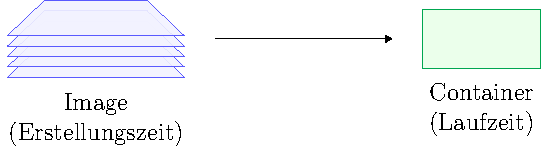
\includegraphics[width=\wMD]{app/container-image-relation.pdf}
    \caption{Die allgemeine Beziehung zwischen
    Docker-Image und Container \parencite[52]{book:docker-dd}}
    \label{fig:container-image-relation}
\end{figure}

\noindent
Der Befehl \consoleinline{docker container create}
wird verwendet, um ein oder mehrere Container von einem Image zu erstellen
und mit \consoleinline{docker container run} alternativ direkt zu starten.
Nachdem ein Container erstellt wurde,
ist dieser fest an das zugrunde liegende Image gebunden.
Das Image kann erst dann gelöscht werden,
wenn es keine Container mehr gibt, die dieses verwenden.
Der Versuch, solches zu entfernen, würde zu einem Fehler führen.
Der restliche Teil dieses Abschnitts wird sich mit den Befehlen beschäftigen,
um die Anwendung zu starten.
Die Docker-Images sind alle zusammen kompatibel mit der ARM64-Architektur
und können daher vollständig auf einem Gerät wie dem
Siemens SIMATIC IOT2050 ausgeführt werden.
Das Bereitstellen einer containerisierten Anwendung ist ein zweiteiliger Prozess:
\begin{enumerate}
  \item Erstelle ein Netzwerk über das die Container kommunizieren.
  \item Lege die Container an und starte und verbinde sie mit dem Netzwerk.
\end{enumerate}
Wird die Anwendung auf einem einzelnen Host ausgeführt, bietet sich
die einfachste Form der Docker-Netzwerke an: dem \textit{single-host bridge network}.
Der Name verrät bereits zwei Dinge \parencite[155]{book:docker-dd}:
\begin{description}[style=nextline]
  \item[Single-Host]
  Das Netz existiert auf einem einzigen Docker-Host und kann auch nur Container
  von diesem Host verbinden.
  \item[Bridge]
  Es handelt sich um eine Implementierung des 802.1d Bridge Standards (Layer-2-Switch).
\end{description}
Der folgende Befehl erstellt ein \textit{single-host bridge network} mit dem Namen
\consoleinline{appnet}:
\begin{consolecode}
$ docker network create --driver bridge appnet
\end{consolecode}
Dieses taucht nun in der Liste der Docker-Netze auf:
\begin{consolecode}
$ docker network ls
NETWORK ID     NAME      DRIVER    SCOPE
2a64863b85ac   appnet    bridge    local
de8bf5113652   bridge    bridge    local
[...]
\end{consolecode}
Zusätzliche wurde auf Linux eine neue \textit{Linux bridge} im Kernel angelegt.
Diese können mit dem \consoleinline{brctl} Befehl aus dem \consoleinline{bridge-utils}
Paket beobachtet werden:
\begin{consolecode}
$ brctl show
bridge name       bridge id           STP enabled   interfaces
br-2a64863b85ac   8000.02421cd6ffff   no
docker0           8000.0242b48f93e6   no
\end{consolecode}
Die Ausgabe zeigt zwei Netzwerkbrücken. Die erste Zeile (\consoleinline{br-2a64863b85ac})
bezieht sich auf die neu angelegte Docker-Brücke \consoleinline{appnet}.
Die zweite Zeile (\consoleinline{docker0}) korrespondiert mit der
von Docker erstellte Standard-Brücke. Keine der beiden Brücken
haben verbundene Geräte (\consoleinline{interfaces} Spalte).
Wir können nun zwei Container erstellen, diese an die \consoleinline{appnet}
Brücke anfügen und ein wenig Konnektivität testen:
\begin{consolecode}
$ docker run -d --network appnet --name c1 alpine sleep 1d
$ docker run -d --network appnet --name c2 alpine sleep 1d
\end{consolecode}
Die vorhergehenden Befehle starten zwei Container mit Basis auf dem
\textit{Alpine Linux} Docker-Image, welches nur rund \qty{5}{\mega\byte} groß ist,
und führen das \consoleinline{sleep 1d} Kommando aus.
Ein Blick in das \consoleinline{appnet} Netz offenbart nun zwei verbundene Container:
\begin{consolecode}
$ docker network inspect appnet
[...]
"Containers": {
  "341ee8dfafa...d0401892a7d": {
    "Name": "c1",
    "EndpointID": "ad3241d27a7...3ba94ca3225",
    "MacAddress": "02:42:ac:12:00:02",
    "IPv4Address": "172.18.0.2/16",
    "IPv6Address": ""
  },
  "8c574b9a71e...7fa033427e9": {
    "Name": "c2",
    "EndpointID": "0f2a5f0dcdd...8dd3d481861",
    "MacAddress": "02:42:ac:12:00:03",
    "IPv4Address": "172.18.0.3/16",
    "IPv6Address": ""
  }
}
[...]
\end{consolecode}
Auch das \consoleinline{brctl} Kommando zeigt nun zwei angeschlossene Interfaces:
\begin{consolecode}
$ brctl show
bridge name       bridge id           STP enabled   interfaces
br-2a64863b85ac   8000.02421cd6ffff   no            veth063da62
                                                    veth3c4e683
docker0           8000.0242b48f93e6   no
\end{consolecode}
Innerhalb einer der Container sollte es nun möglich sein, den jeweils
anderen Container per Name zu erreichen.
Dies funktioniert deshalb, da alle Container automatisch
beim eingebetteten Docker DNS Dienst registriert werden
und so die Namen aller Container
im selben Netzwerk auflösen können \parencite[160]{book:docker-dd}.
Die folgenden Befehle testen die Verbindung:
\begin{consolecode}
$ # Bringe eine Shell an Container eins an
$ docker exec -it c1 sh
(c1) $ # Ein Ping zu Container zwei per Name sollte funktionieren
(c1) $ ping c2 -c 2
PING c2 (172.18.0.3): 56 data bytes
64 bytes from 172.18.0.3: seq=0 ttl=64 time=0.582 ms
64 bytes from 172.18.0.3: seq=1 ttl=64 time=0.279 ms
\end{consolecode}
Die Namensauflösung funktioniert